\section{Conceptual Model for SDD}

\subsection{Software Design Context}
Our project will be composed of various software pipelines that need to be interfaced together in order to have a contiguous reliable model. In order to accomplish this we need to lay out all the required components and explore how they can interface between each other. Furthermore, if a workaround is necessary then we need to outline it and warn the user of potential pitfalls and drawbacks. At the heart of the project we will be utilizing a raspberry PI which will coordinate the various software components required for the build. The raspberry pi will be running on the raspbian OS. As we will need to train the neural network, data will need to be collected and stored, as the raspberry pi has limited storage we will be mounting an external hard drive to it. Moreover this external hard drive will have to be connected to a database, in this case we will be using SQLite. Next, we will be using a USB webcam to take pictures and store them on the external hard drive attached to the raspberry pi. The external hard drive will also be used to store the processed training data that will also be attached to an external computer with the necessary resources needed to train the network, namely a powerful Nvidia GPU running CUDA drivers. Training will be done through the Keras deep learning framework and the resulting neural network model will be stored into a movidius compute stick as a .h5 file. Finally, we will be utilizing the aforementioned Intel Movidius Neural Compute Stick running NCSDK to classify the real time images taken by the webcam, and the images will be stored in the external hard drive and referenced to by the database with the right classification.

\subsection{SDD Life Cycle}
Our first step will be to manually capture images through the raspberry pi and a usb webcam and store them on an external hard drive. Once the images are taken we will use a python script with the opencv library to segment the image into individual seeds and manually classify/label each one, and store them once again into the library into labeled training/validation directories while deleting the original image. Because we have the properly labeled data, we will write another piece of software utilizing the Keras library to develop the Convolutional Neural Network architecture and train it on a GPU, using the directories we created earlier. The resulting trained matrix will be stored as a .h5 file on the Movidius VPU computer stick. This process is just to train the network for future product integration.

\begin{figure}[h]
\caption(Training Workflow Diagram)
\centering
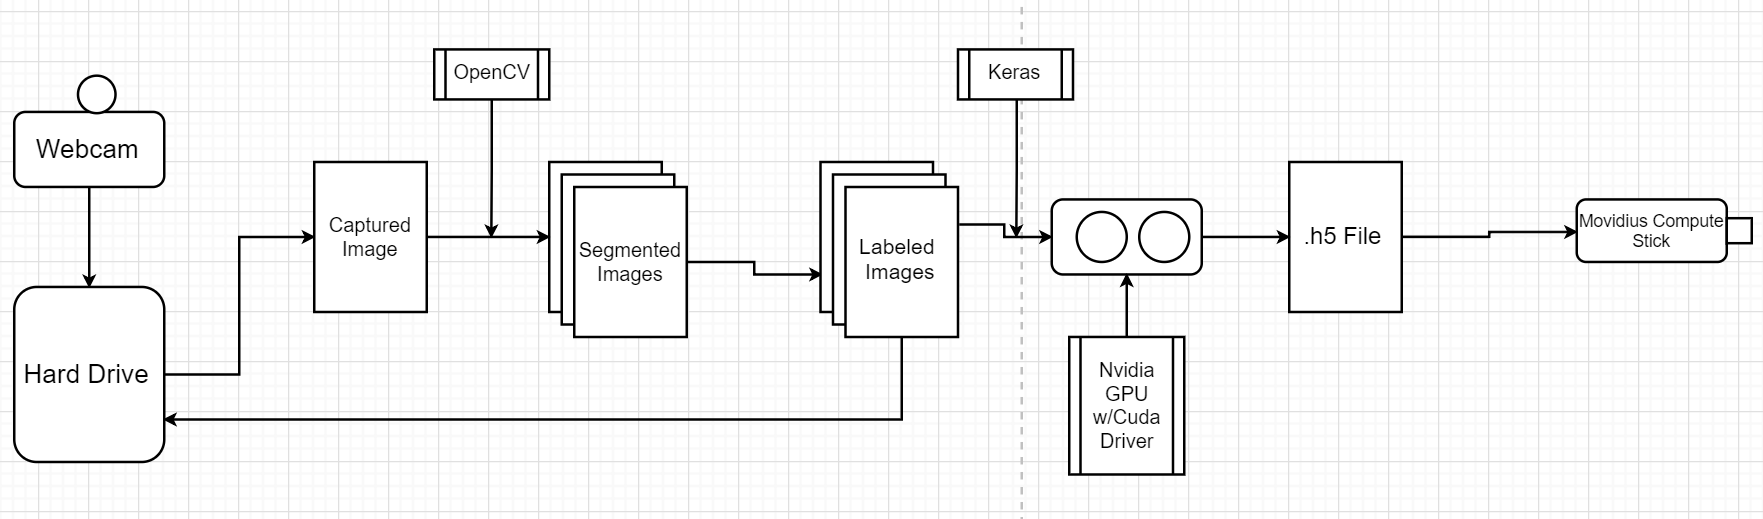
\includegraphics[height=6cm]{Trainingseeddiagram}
\end{figure}

The initial steps in our final product is similar to the training process. We start with the capturing of images and segment them in the same python script using opencv. The partitioned images with individual seeds are stored into a specified folder for classification. A separate python program will be developed with the .h5 file from the compute stick loaded to classify images fed through the hard drive, the output of the classification will be sent to two external sources. One, back to the hard drive with references to the images to be stored onto the database, two the output will be sent to another python program, that will invoke a system call to light up an LED if a bad seed is detected.

\begin{figure}[h]
\caption(Raspberry Pi Diagram)
\centering
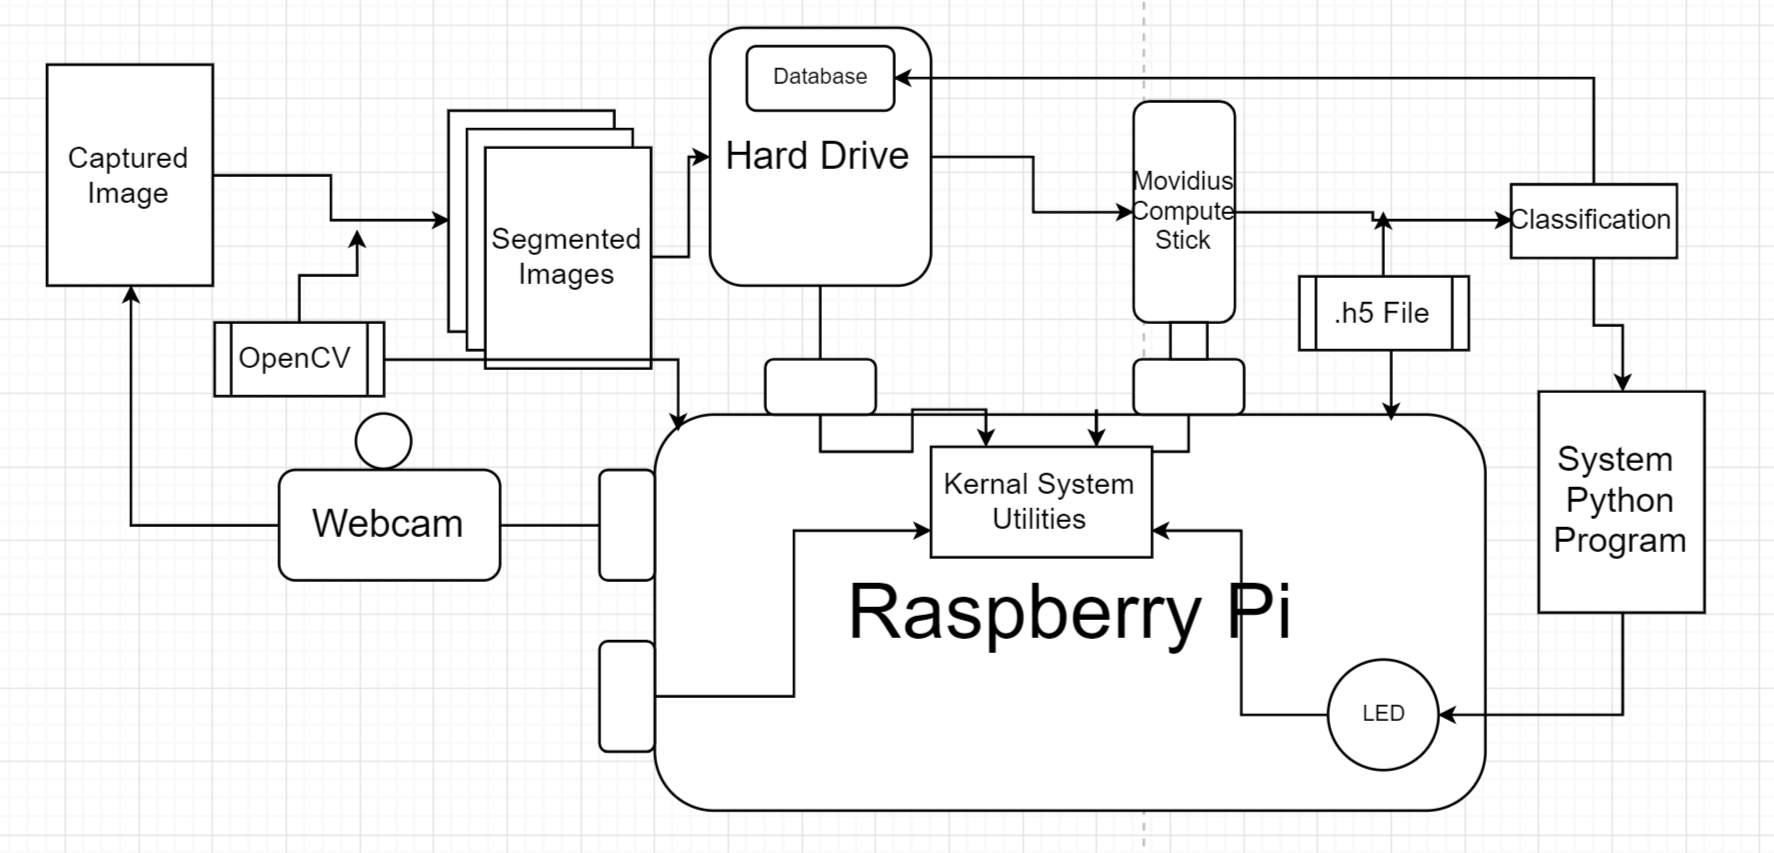
\includegraphics[height=6cm]{Raspiseeddiagram}
\end{figure}
